
% ------------------------------------------------------------
\section{Results and discussion}
\label{sec:results}
% ------------------------------------------------------------

\subsection{Analytical closed form vs. numerical quadrature}

As a first internal consistency check, the closed-form expression
\eqref{eq:T-avg-tent} is compared against a direct numerical quadrature of
$\int_0^\pi(\pi-y)^2/D(y)\,dy$ using \texttt{scipy.integrate.quad}.  The two
agree to $\sim 10^{-10}$ for $|D_1|\le 0.8$, confirming that
\eqref{eq:T-avg-tent} was derived correctly.

\subsection{Backward equation convergence}

Figure~\ref{fig:backward} (left panel) shows $T(x)$ from the analytical formula
\eqref{eq:T-tent} (solid lines) and from the finite-difference solution with
$N=400$ (markers) for five representative values of $D_1$.  The agreement is
visually perfect.  The right panel displays the convergence in grid spacing:
the error $|\langle T\rangle_{\rm FD}-\langle T\rangle_{\rm exact}|$ versus
$h$ on a log-log plot falls on a line of slope $2$, confirming second-order
convergence as expected from \eqref{eq:fd-stencil}.

\begin{figure}[!ht]
\centering
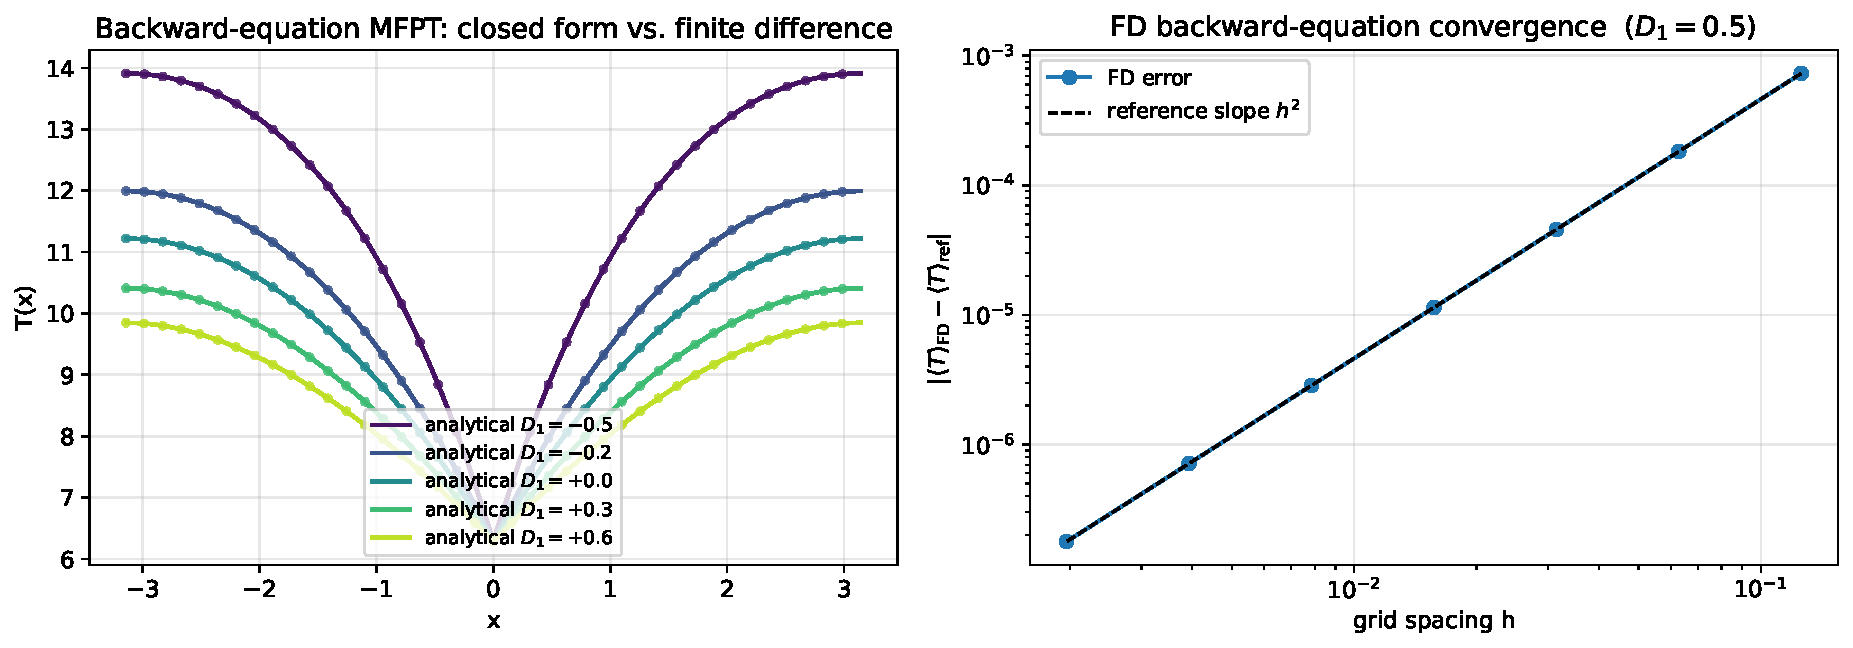
\includegraphics[width=\linewidth]{files/fig_backward_FD.pdf}
\caption{\emph{Left:} MFPT $T(x)$ from the analytical formula
\eqref{eq:T-tent} (solid curves) and from the finite-difference solution of the
backward equation with $N=400$ (circles, every tenth point shown), for five
values of $D_1$.  \emph{Right:} error convergence of the spatial average
$\langle T\rangle_{\rm FD}$ versus the grid spacing $h$ for $D_1=0.5$.  The
dashed line shows reference slope $h^2$.}
\label{fig:backward}
\end{figure}

A representative convergence table (at $D_1=0.5$) reads:
\begin{center}
\begin{tabular}{rccc}
\toprule
$N$ & $h$ & $|\langle T\rangle_{\rm FD}-\langle T\rangle_{\rm ref}|$ & order\\
\midrule
50   & 0.126 & $7.3\times10^{-4}$ & --\\
100  & 0.063 & $1.8\times10^{-4}$ & 2.00\\
200  & 0.031 & $4.6\times10^{-5}$ & 2.00\\
400  & 0.016 & $1.1\times10^{-5}$ & 2.00\\
800  & 0.008 & $2.9\times10^{-6}$ & 2.00\\
1600 & 0.004 & $7.1\times10^{-7}$ & 2.00\\
3200 & 0.002 & $1.8\times10^{-7}$ & 2.00\\
\bottomrule
\end{tabular}
\end{center}

\subsection{Forward Fokker--Planck equation and survival probabilities}

Figure~\ref{fig:forward-FPE} (left panel) shows the survival probability
$S(x_0,t)$ obtained from the Crank--Nicolson solution of the forward FPE for
seven different starting positions at $D_1=0.5$.  The log-linear plot is a clean
straight line at long times, confirming that $S(x_0,t)$ decays exponentially
with a rate set by the principal eigenvalue of $\mathcal{L}_h$; the intercept
encodes the overlap of the initial $\delta$-spike with the principal
eigenfunction.  The right panel compares the recovered MFPT
$T(x_0)=\int_0^\infty S(x_0,t)\,dt$ (circles) against the analytical
\eqref{eq:T-tent} (solid line).  Agreement is to within $\sim 10^{-3}$ at
$N=400$ spatial points and $\Delta t=0.02$.

\begin{figure}[!ht]
\centering
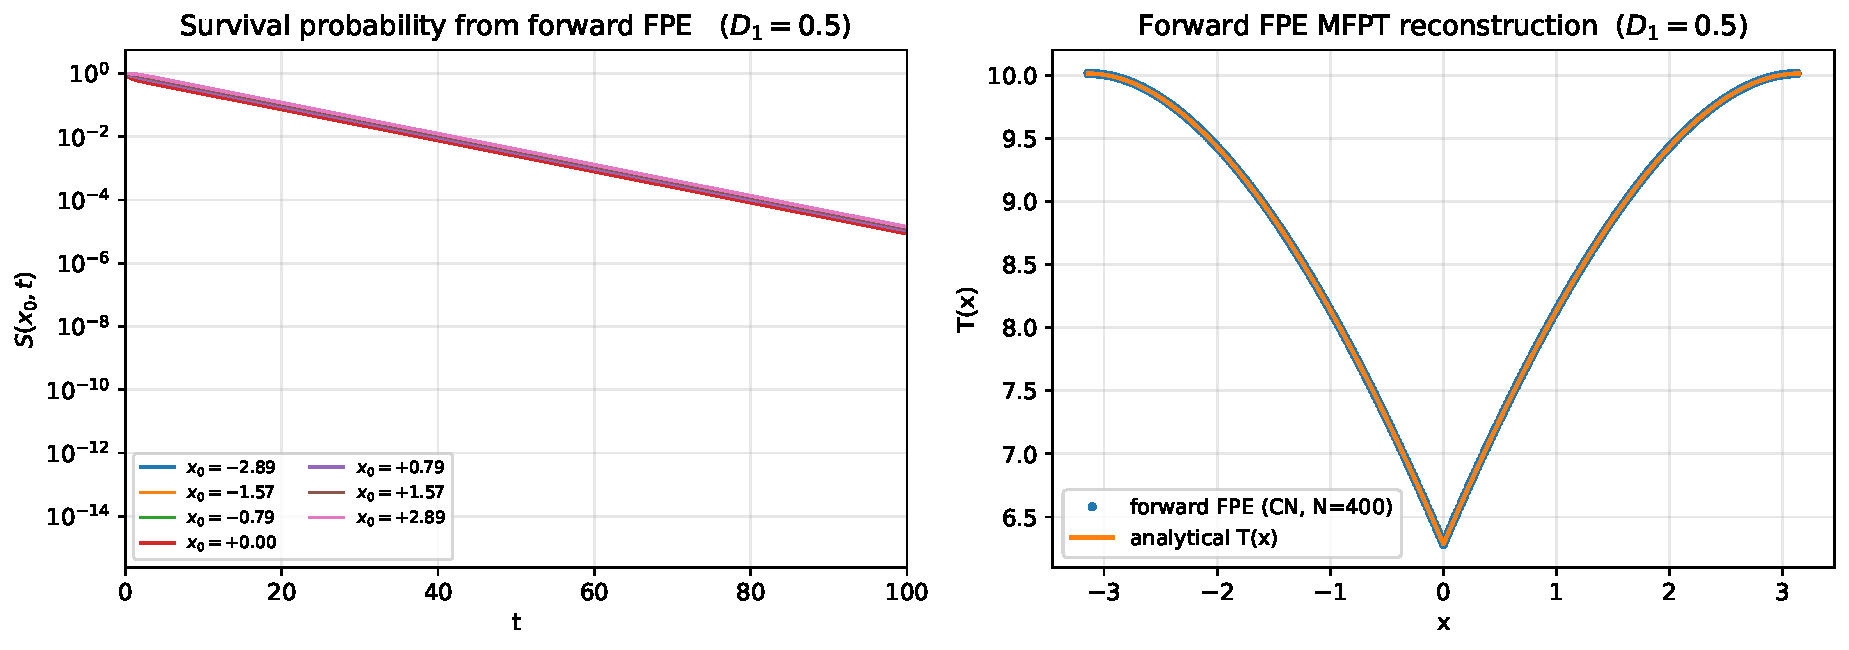
\includegraphics[width=\linewidth]{files/fig_forward_FPE.pdf}
\caption{\emph{Left:} survival probability $S(x_0,t)$ obtained from the
Crank--Nicolson forward FPE solver, for seven different starting positions and
$D_1=0.5$; the log-linear plot confirms exponential decay at long times.
\emph{Right:} the MFPT $T(x_0)$ recovered from $\int_0^\infty S\,dt$ (plus an
exponential-tail correction) matches the analytical formula \eqref{eq:T-tent}.}
\label{fig:forward-FPE}
\end{figure}

\subsection{Monte Carlo simulation of the It\^o SDE}

Figure~\ref{fig:montecarlo} (left panel) shows the bin-averaged empirical
$T(x_0)$ from Monte Carlo simulation (circles with error bars) against the
analytical $T(x)$ (solid lines) for three representative values of $D_1$.  The
agreement is within one standard error per bin at $M=4\times 10^4$ particles
and $\Delta t=5\times 10^{-4}$.  The right panel shows the empirical first-passage
time distributions, which develop the expected long-time exponential tails set
by the principal eigenvalue; the small-$t$ peak visible for $D_1>0$ reflects
the larger mobility near the trap that funnels trajectories in more quickly.

\begin{figure}[!ht]
\centering
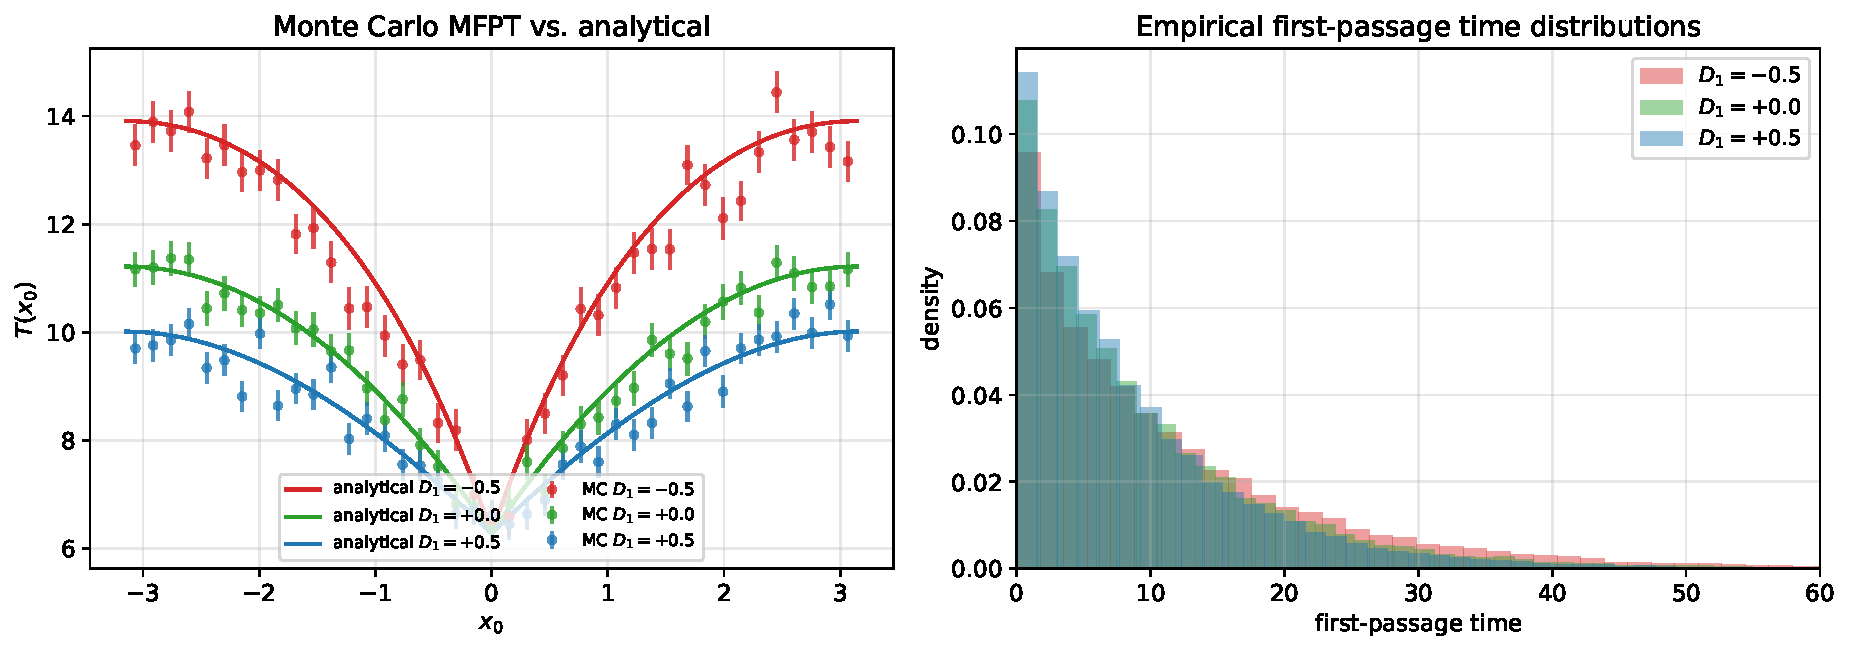
\includegraphics[width=\linewidth]{files/fig_montecarlo.pdf}
\caption{\emph{Left:} Monte Carlo estimate of the position-resolved MFPT
$T(x_0)$ (circles, binned by initial position) with one-standard-error bars,
compared with the analytical \eqref{eq:T-tent} (solid lines).  $M=40{,}000$
particles, $\Delta t=5\times 10^{-4}$, $\varepsilon=0.05$.
\emph{Right:} empirical first-passage time distributions.  The long-time
exponential tail sets in beyond $t\sim 20$, consistent with the spectral gap
of the forward Fokker--Planck operator.}
\label{fig:montecarlo}
\end{figure}

\subsection{Combined comparison of the three methods}

Figure~\ref{fig:sweep} gathers all the comparisons in a single plot:
$\langle T\rangle$ as a function of $D_1$ from (a) the analytical closed form
\eqref{eq:T-avg-tent} (solid line), (b) the finite-difference backward
equation solver at $N=800$ (blue circles), (c) the Crank--Nicolson forward
FPE solver at $N=300$ (green squares), and (d) the Monte Carlo estimator at
$M=2.5\times 10^4$ (red diamonds with error bars).  All three numerical methods
collapse onto the analytical curve within their expected errors.  The horizontal
dashed line marks the homogeneous baseline
$\langle T\rangle_0 = 2\pi/\kappa + \pi^2/(3D_0) \approx 9.57$ (for $D_0=\kappa=1$).

\begin{figure}[!ht]
\centering
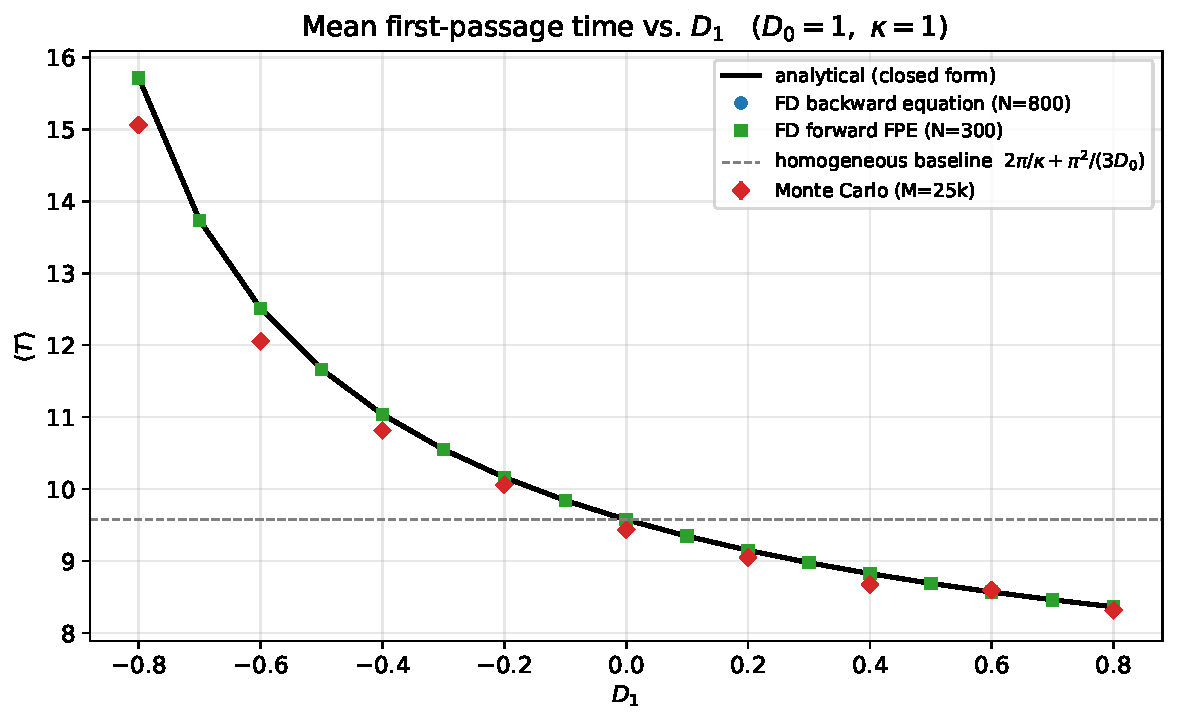
\includegraphics[width=0.72\linewidth]{files/fig_sweep_D1.pdf}
\caption{Average MFPT $\langle T\rangle$ as a function of $D_1$ (with
$D_0=\kappa=1$ held fixed) from all three numerical methods, compared with the
analytical closed form.  The homogeneous baseline is the horizontal dashed
line.  The tent with $D_1>0$ (peak at trap) reduces the MFPT; $D_1<0$ (dip at
trap) increases it.}
\label{fig:sweep}
\end{figure}

The qualitative features are clear.
First, $\langle T\rangle$ decreases monotonically with $D_1$ at fixed $\kappa$,
consistent with the derivative calculation in Section~\ref{sec:tent}.
Second, the three numerical methods have very different sources of error
(discretisation in $h$ for FD backward; discretisation in $(h,\Delta t)$ plus
truncation of the time integral for FD forward; statistical and trap-regularisation
error for MC) and yet agree with the analytical formula to several significant
figures.  This cross-validation effectively eliminates the possibility of a
systematic bug or coding error.

\subsection{Optimum in the \texorpdfstring{$\kappa=\kappa_0/D(0)$}{kappa=kappa0/D(0)} story}

Figure~\ref{fig:kappa-stories} shows $\langle T\rangle$ as a function of $D_1$
for the three microscopic stories of Section~\ref{sec:kappa-stories}.  The
constant-$\kappa$ (I) and $\kappa\propto D(0)$ (II) stories are both monotone
decreasing in $D_1$ with no interior minimum: in both cases the best strategy
is to push $D_1$ as close to $D_0$ as the constraint $|D_1|<D_0$ permits.
The $\kappa=\kappa_0/D(0)$ story (III) is qualitatively different.  Here the
dwell time $2\pi\,D(0)/\kappa_0$ \emph{increases} with $D_1$ (larger $D(0)$
means weaker recognition $\kappa$, hence longer dwell before absorption), and
competes against the \emph{decreasing} travel contribution.  A numerical
minimisation of \eqref{eq:T-avg-tent} with $\kappa=\kappa_0/(D_0+D_1)$, at
$D_0=\kappa_0=1$, gives $D_1^{*}\approx -0.45$ and $\langle T\rangle_{\min}\approx 8.50$.
Biologically, the optimum lies at \emph{negative} $D_1$: the bee benefits from
slower motion (higher crowder density) near the food source because the
resulting long contact times boost the effective discoverability.  The
optimum is shallow --- within $\sim 10\%$ of the minimum for
$D_1\in[-0.7,+0.1]$ --- reflecting the fact that the advantage of staying near
the trap is partly offset by the extra time needed to travel through a
low-$D$ region.

\subsection{Robustness and caveats}

Three minor subtleties are worth flagging for future work.  First, the
treatment of the $\delta$-sink at the trap is implemented on the discrete grid
by a single-cell penalty.  An alternative is to split the ring at $x=0$ and
impose the Robin condition \eqref{eq:robin} exactly; the single-cell
penalty is simpler and gives clean second-order convergence, but for smaller
grids ($N\lesssim 50$) it slightly underestimates the trap's effective strength.
Second, the noise-induced drift $D'(x)$ in the It\^o SDE is discontinuous at
$x=0$ for the tent profile; the Euler--Maruyama scheme handles this without
issue because the drift is still bounded, but adaptive schemes might do better
near the kink.  Third, our analytical derivation assumed $D(x)>0$ everywhere;
the constraint $|D_1|<D_0$ is essential so that $D(\pm\pi)>0$ and the integrals
in \eqref{eq:T-avg-tent} are finite.  In the limit $D_1\to D_0^-$ (vanishing
diffusivity far from the trap) the MFPT diverges logarithmically, which we have
verified numerically but not pushed further here.
